\documentclass[11pt]{article}
\usepackage[utf8]{inputenc}
\usepackage[english]{babel}
\usepackage{bilal2vec}
\usepackage{minted}
\title{CS 486 - Assignment 4}
\author{Bilal Khan\\
\href{mailto:bilal2vec@gmail.com}{bilal2vec@gmail.com}}
\date{\today}

\begin{document}

\maketitle
\tableofcontents

I used the cursor (cursor.com) code editor to help write the code for this assignment.

\section{1}

\subsection{a}

A textual form of the BN is:

Variables: D (Dunetts), T (TRIMONO), S (Sloepnea), F (Foriennditis), G (Degar)

D states: 0 (None), 1 (Mild), 2 (Severe)

T, S, F, G states: 0 (Absent), 1 (Present)

Structure: $D \rightarrow S$, $T \rightarrow S$, $D \rightarrow F$, $D \rightarrow G$

\subsection{b}

\begin{minted}{python}
import numpy as np
import matplotlib.pyplot as plt
import copy
from tqdm import tqdm

initial_cpts = {
    'D': np.array([0.5, 0.25, 0.25]),
    'T': np.array([0.9, 0.1]),
}

initial_cpts_f = {  #P(F|D)
    (0,): 0.2,
    (1,): 0.8,
    (2,): 0.2,
}

initial_cpts_g = {  #P(G|D)
    (0,): 0.2,
    (1,): 0.2,
    (2,): 0.8,
}

initial_cpts_s = {  #P(S|D,T)
    (0, 0): 0.2,
    (1, 0): 0.8,
    (2, 0): 0.8,
    (0, 1): 0.01,
    (1, 1): 0.01,
    (2, 1): 0.01,
}


def expand_cpt(cpt_dict):
    full_cpt = {}
    for key, p_state1 in cpt_dict.items():
        full_cpt[key] = np.array([1.0 - p_state1, p_state1])
    return full_cpt


initial_cpts['F'] = expand_cpt(initial_cpts_f)
initial_cpts['G'] = expand_cpt(initial_cpts_g)
initial_cpts['S'] = expand_cpt(initial_cpts_s)


def load_data(filename):
    data = np.loadtxt(filename, dtype=int)
    return data


def add_noise(cpts, delta):
    noisy_cpts = copy.deepcopy(cpts)

    noise_d = np.random.uniform(0, delta, size=noisy_cpts['D'].shape)
    noisy_cpts['D'] = noisy_cpts['D'] + noise_d
    noisy_cpts['D'] /= noisy_cpts['D'].sum()

    # not noising t

    for node in ['F', 'G', 'S']:
        for key in noisy_cpts[node]:
            noise = np.random.uniform(0,
                                      delta,
                                      size=noisy_cpts[node][key].shape)
            noisy_cpts[node][key] = noisy_cpts[node][key] + noise
            noisy_cpts[node][key] /= noisy_cpts[node][key].sum()

    return noisy_cpts


def get_prob(cpt_entry, state):
    return cpt_entry[state]


def e_step(data, cpts):
    num_patients = data.shape[0]
    num_states = 3
    weights = np.zeros((num_patients, num_states))

    for i in range(num_patients):
        patient = data[i]
        s_val, f_val, g_val, t_val, d_known = patient[0], patient[1], patient[
            2], patient[3], patient[4]

        if d_known != -1:
            weights[i, d_known] = 1.0
        else:
            unnormalized_probs = np.zeros(num_states)
            for d_state in range(num_states):
                prob_s_dt = get_prob(cpts['S'][(d_state, t_val)], s_val)
                prob_f_d = get_prob(cpts['F'][(d_state,)], f_val)
                prob_g_d = get_prob(cpts['G'][(d_state,)], g_val)
                prob_d = get_prob(cpts['D'], d_state)
                unnormalized_probs[
                    d_state] = prob_s_dt * prob_f_d * prob_g_d * prob_d

            total_prob = unnormalized_probs.sum()
            if total_prob > 1e-8:
                weights[i, :] = unnormalized_probs / total_prob
            else:
                weights[i, :] = 1.0 / num_states

    return weights


def m_step(data, weights):
    num_patients = data.shape[0]
    num_states = 3
    new_cpts = copy.deepcopy(initial_cpts)

    total_weights = weights.sum(axis=0)
    new_cpts['D'] = total_weights / num_patients

    t_counts = np.zeros(2)
    for i in range(num_patients):
        t_val = data[i, 3]
        t_counts[t_val] += weights[i].sum()
    t_present_count = np.sum(data[:, 3] == 1)
    new_cpts['T'] = np.array(
        [1.0 - t_present_count / num_patients, t_present_count / num_patients])

    f_counts = {}
    for d_state in range(num_states):
        f_counts[(d_state,)] = np.zeros(2)

    for i in range(num_patients):
        f_val = data[i, 1]
        for d_state in range(num_states):
            f_counts[(d_state,)][f_val] += weights[i, d_state]

    for d_state in range(num_states):
        total_d_weight = f_counts[(d_state,)].sum()
        if total_d_weight > 1e-8:
            new_cpts['F'][(d_state,)] = f_counts[(d_state,)] / total_d_weight
        else:
            new_cpts['F'][(d_state,)] = np.array([0.5, 0.5])

    g_counts = {}
    for d_state in range(num_states):
        g_counts[(d_state,)] = np.zeros(2)

    for i in range(num_patients):
        g_val = data[i, 2]
        for d_state in range(num_states):
            g_counts[(d_state,)][g_val] += weights[i, d_state]

    for d_state in range(num_states):
        total_d_weight = g_counts[(d_state,)].sum()
        if total_d_weight > 1e-8:
            new_cpts['G'][(d_state,)] = g_counts[(d_state,)] / total_d_weight
        else:
            new_cpts['G'][(d_state,)] = np.array([0.5, 0.5])

    s_counts = {}
    for d_state in range(num_states):
        for t_state in range(2):
            s_counts[(d_state, t_state)] = np.zeros(2)

    for i in range(num_patients):
        s_val, t_val = data[i, 0], data[i, 3]
        for d_state in range(num_states):
            s_counts[(d_state, t_val)][s_val] += weights[i, d_state]

    for d_state in range(num_states):
        for t_state in range(2):
            total_dt_weight = s_counts[(d_state, t_state)].sum()
            if total_dt_weight > 1e-8:
                new_cpts['S'][(
                    d_state,
                    t_state)] = s_counts[(d_state, t_state)] / total_dt_weight
            else:
                new_cpts['S'][(d_state, t_state)] = np.array([0.5, 0.5])

    return new_cpts


def llh(data, weights, cpts):
    log_likelihood = 0.0
    num_patients = data.shape[0]
    num_states = 3

    log_cpts = copy.deepcopy(cpts)
    log_cpts['D'] = np.log(log_cpts['D'] + 1e-8)
    log_cpts['T'] = np.log(log_cpts['T'] + 1e-8)
    for node in ['F', 'G', 'S']:
        for key in log_cpts[node]:
            log_cpts[node][key] = np.log(log_cpts[node][key] + 1e-8)

    for i in range(num_patients):
        patient = data[i]
        s_val, f_val, g_val, t_val = patient[0], patient[1], patient[
            2], patient[3]
        patient_ll = 0.0
        for d_state in range(num_states):
            if weights[i, d_state] > 1e-8:
                log_prob_d = get_prob(log_cpts['D'], d_state)
                log_prob_t = get_prob(log_cpts['T'], t_val)
                log_prob_s_dt = get_prob(log_cpts['S'][(d_state, t_val)], s_val)
                log_prob_f_d = get_prob(log_cpts['F'][(d_state,)], f_val)
                log_prob_g_d = get_prob(log_cpts['G'][(d_state,)], g_val)

                log_joint = log_prob_s_dt + log_prob_f_d +
                  log_prob_g_d + log_prob_t + log_prob_d
                patient_ll += weights[i, d_state] * log_joint

        log_likelihood += patient_ll

    return log_likelihood


def run_em(train_data, initial_cpts, convergence_threshold, max_iterations=10):
    cpts = copy.deepcopy(initial_cpts)
    prev_llh = -np.inf
    iterations = 0

    for _ in range(max_iterations):
        weights = e_step(train_data, cpts)
        cpts = m_step(train_data, weights)

        current_llh = llh(train_data, weights, cpts)
        llh_dif = abs(current_llh - prev_llh)

        if llh_dif < convergence_threshold:
            break

        prev_llh = current_llh
        iterations += 1

    return cpts


def predict(patient_data, cpts):
    num_states = 3
    posterior_probs = np.zeros(num_states)
    s_val, f_val, g_val, t_val = patient_data[0], patient_data[1], patient_data[
        2], patient_data[3]

    for d_state in range(num_states):
        prob_s_dt = get_prob(cpts['S'][(d_state, t_val)], s_val)
        prob_f_d = get_prob(cpts['F'][(d_state,)], f_val)
        prob_g_d = get_prob(cpts['G'][(d_state,)], g_val)
        prob_d = get_prob(cpts['D'], d_state)
        posterior_probs[d_state] = prob_s_dt * prob_f_d * prob_g_d * prob_d

    prediction = np.argmax(posterior_probs)
    return prediction


def calculate_acc(test_data, cpts):
    n_correct = 0
    n_total = test_data.shape[0]

    for i in range(n_total):
        patient = test_data[i]
        true_d_state = patient[4]
        predicted_d_state = predict(patient, cpts)
        if predicted_d_state == true_d_state:
            n_correct += 1

    acc = n_correct / n_total
    return acc


def run_experiment(train_file, test_file, initial_cpts_base):
    train_data = load_data(train_file)
    test_data = load_data(test_file)

    delta_values = np.linspace(0.0, 4.0, 20)
    num_trials = 20
    convergence_thresh = 0.05

    results_before_em = {delta: [] for delta in delta_values}
    results_after_em = {delta: [] for delta in delta_values}

    for delta in tqdm(delta_values):
        for trial in range(num_trials):
            noisy_initial_cpts = add_noise(initial_cpts_base, delta)

            accuracy_before = calculate_acc(test_data, noisy_initial_cpts)
            results_before_em[delta].append(accuracy_before)

            learned_cpts = run_em(train_data, noisy_initial_cpts,
                                  convergence_thresh)

            accuracy_after = calculate_acc(test_data, learned_cpts)
            results_after_em[delta].append(accuracy_after)

    mean_before = [np.mean(results_before_em[d]) for d in delta_values]
    std_before = [np.std(results_before_em[d]) for d in delta_values]
    mean_after = [np.mean(results_after_em[d]) for d in delta_values]
    std_after = [np.std(results_after_em[d]) for d in delta_values]

    plt.figure(figsize=(10, 6))
    plt.errorbar(delta_values,
                 mean_before,
                 yerr=std_before,
                 label='Accuracy Before EM',
                 fmt='-o',
                 capsize=5)
    plt.errorbar(delta_values,
                 mean_after,
                 yerr=std_after,
                 label='Accuracy After EM',
                 fmt='-s',
                 capsize=5)

    plt.xlabel('Noise Level (δ)')
    plt.ylabel('Prediction Accuracy on Test Set')
    plt.title('EM Sensitivity to Initial CPT Noise')
    plt.legend()
    plt.grid(True)
    plt.ylim(0, 1.05)
    plot_filename = 'em_accuracy_vs_delta.png'
    plt.savefig(plot_filename)
    print(f"\nPlot saved to {plot_filename}")

    return plot_filename


if __name__ == "__main__":
    train_filename = 'traindata.txt'
    test_filename = 'testdata.txt'
    plot_file = run_experiment(train_filename, test_filename, initial_cpts)
\end{minted}

\subsection{c}

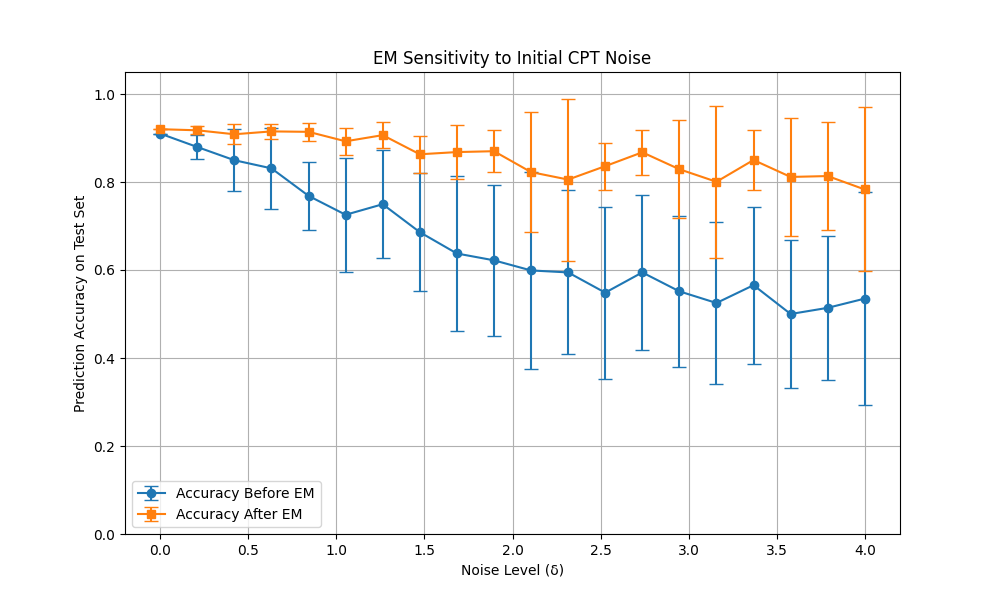
\includegraphics[width=1.0\textwidth]{em_accuracy_vs_delta.png}

\end{document}